% !TEX root =  ../../../master.tex
\subsection{Docker}
\label{sec:grundlagen:docker}
Bei heutiger Softwareentwicklung spielt die Art und Weise, wie eine Software bereitgestellt wird, eine zentrale Rolle. 
Gerade bei der Entwicklung einer verteilten Architektur wie die der Microservices\footnote{siehe \ref{ch:microservice}} ist dies besonders wichtig, da die einzelnen Schritte dieses Prozesses weitestgehend automatisch durchgeführt werden sollen. 
Weiterhin benötigen Microservices in der Regel nur sehr wenige Hardware-Ressourcen und arbeiten autonom. 
Aus diesen Gründen ist es sinnvoll die vorhandenen Ressourcen eines Servers sinnvoll zu verteilen und gleichzeitig eine isolierte Umgebung für die einzelnen Microservices zu schaffen.

Hierbei hat sich in den letzten Jahren der Begriff bzw. die Technologie Docker besonders etabliert.
Docker ist eine von dem Unternehmen Docker Inc. entwickelte Software, welche eine Art der Container-Virtualisierung ermöglicht. 
Die Software baut dabei auf eine Vielzahl von Open-Source-Projekten auf.

Die Container-Virtualisierung ist eine leichtgewichtige und ressourcenschonende Variante der Virtualisierung von Arbeitsumgebungen für Anwendungen. 
Im Gegensatz zu virtuellen Maschinen bilden Container kein eigenständiges System ab, welches über virtuelle Hardware und ein vollständiges Betriebssystem verfügt. 
Vielmehr wird eine isolierte Umgebung für eine spezifische Anwendung zur Verfügung gestellt, welche die Ressourcen des zugrundeliegenden Systems verwenden. 

\begin{figure}[h]
	\centering
	\captionsetup{justification=centering, format=plain}
	\subfigure[Container-Virtualisierung]{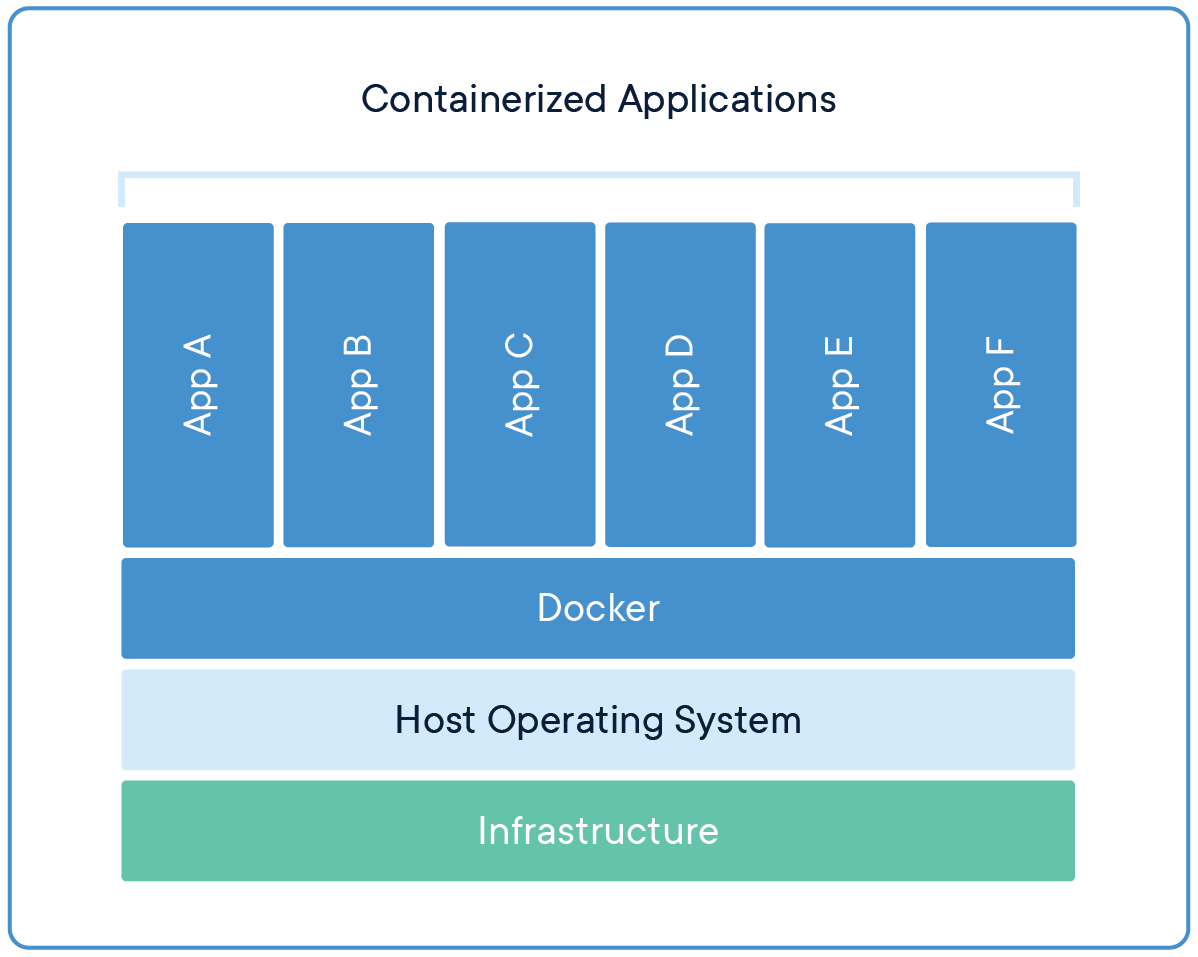
\includegraphics[width=0.45\textwidth]{img/grundlagen/technisch/docker_container}}\hspace{1cm}
	\subfigure[Virtuelle Maschine]{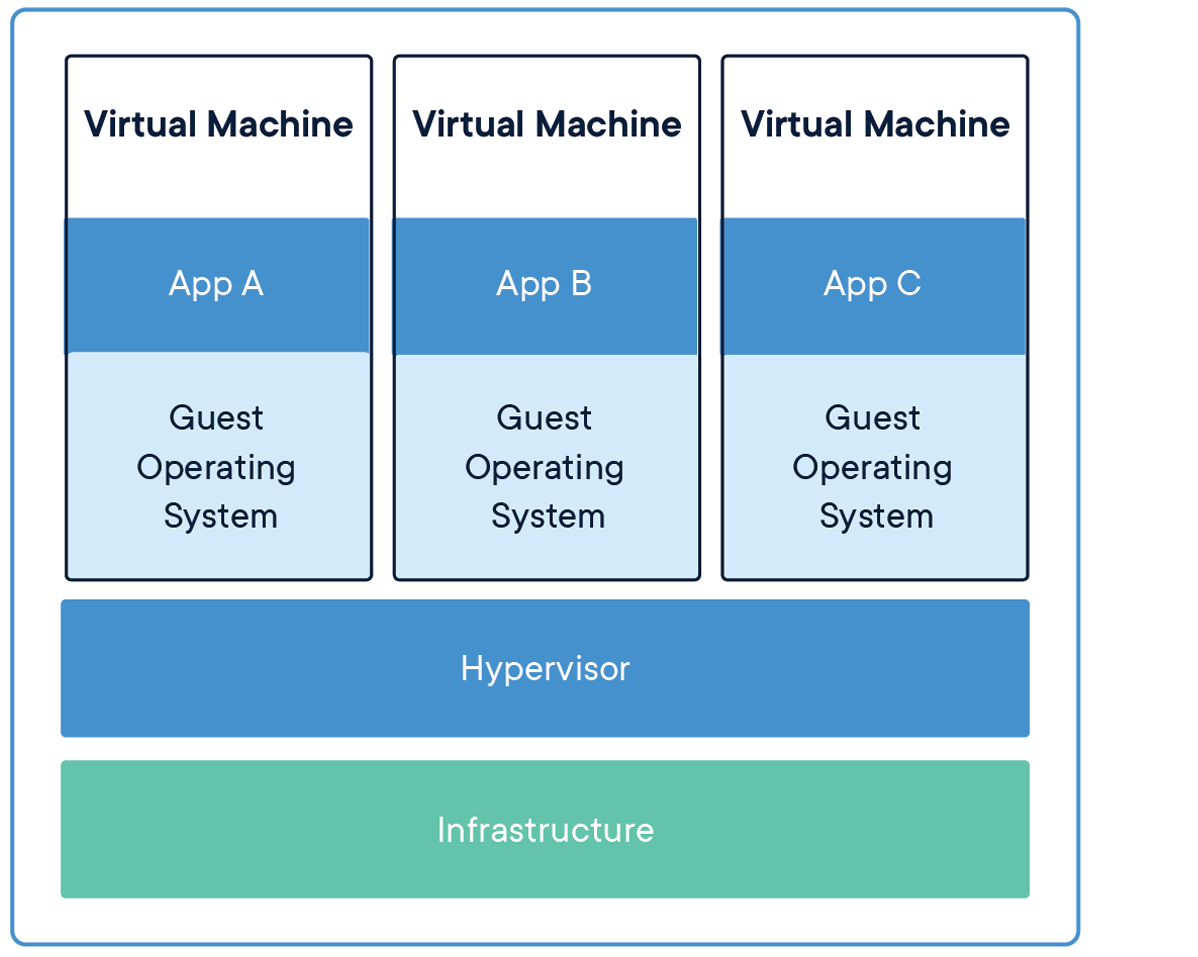
\includegraphics[width=0.45\textwidth]{img/grundlagen/technisch/docker_hypervisor}}
	\caption[Vergleich Container-Virtualisierung vs. virtuelle Maschine]{\label{fig:docker_container}Vergleich Container-Virtualisierung vs. virtuelle Maschine, \\Quelle: \cite{MS-DockerInc..05.03.2019}}
\end{figure}

Abbildung \ref{fig:docker_container} visualisiert die Architektur einer Container-Virtualisierung und zeigt einen Vergleich zur Hardware-Virtualisierung.\autocite[Vgl.][]{MS-ChrissiKraus.27.07.2018}$^,$\autocite[Vgl.][]{MS-MicrosoftCorporation.31.08.2018} 
Wie zu sehen ist, setzt Docker auf dem zugrunde liegenden Betriebssystem auf, wohingegen eine virtuelle Maschine als Gast-System agiert. 
Dabei verwaltet und verteilt bei virtuellen Maschinen ein Hypervisor die Ressourcen, welche die Betriebssysteme zur Verfügung gestellt bekommen. 
Ein Hypervisor ist also ein Manager für virtuelle Maschinen\autocite[Vgl.][]{MS-ReneBust.06.04.2010}. 
Docker-Container bekommen hingegen ihrere Ressourcen vom zugrundeliegenden Betriebssystem bereitgestellt.

Vorteile von Docker sind zum einen das hohe Maß an Integration und zum anderen eine gute Skalierbarkeit von Anwendungen. 
Dabei können die Docker-Container sehr einfach erzeugt, gestartet und gestoppt. 
Als Kern- und Steuerprogramm von Docker fungiert die sogenannte Docker-Engine. 
Sie ist neben dem Starten und Stoppen in der Lage vorhandene Container zu replizieren bzw. die Anzahl an Containern für einen speziellen Dienst bei Bedarf beliebig zu erhöhen oder zu verringern.
Hierzu kommt das Nebenprodukt Docker-Compose zum Einsatz. 
Dieses Werkzeug dient dem Erzeugen von Multi-Container-Anwendungen.
Der Integrationsaspekt entsteht dadurch, dass Docker mit anderer Software interagieren bzw. sich von dieser steuern lassen kann.\autocite[Vgl.][]{MS-Docker-Compose} 